\documentclass[preprint,12pt]{elsarticle} %Change later to review, not preprint

\usepackage{amssymb}
\usepackage{graphics}
\usepackage{float}


\graphicspath{{./Images/}}

\journal{Solar Energy Materials \& Solar Cells}

\begin{document}

\begin{frontmatter}

\title{Life Cycle Analysis of an Adaptive Solar Facade} 


\author[ita]{P. Jayathissa\corref{cor2} \tnoteref{t1}}
    \ead{jayathissa@arch.ethz.ch}

\author[ita]{M. Jansen\tnoteref{t1}}
    %\ead{m.jansen@student.ethz.ch}

\author[baug]{N. Heeren}
    \ead{heeren@ifu.baug.ethz.ch}

\author[baug]{S. Hellweg}
	%∫\ead{hellweg@ifu.baug.ethz.ch}

\author[ita]{A. Schlueter \corref{cor1} }
    \ead{schlueter@arch.ethz.ch}


\tnotetext[t1]{This document is a collaborative effort.} 
\cortext[cor1]{Corresponding author} 
\cortext[cor2]{Principal corresponding author}

\address[ita]{Architecture and Building Systems, Institute of Technology in Architecture,\\ ETH Zurich, Switzerland} 
\address[baug]{Ecological System Design, Institute of Environmental Engineering,\\ ETH Zurich, Switzerland}

\begin{abstract}
Text 
\end{abstract}

\begin{keyword}
Adaptive Solar Facade \sep Life Cycle Analysis \sep Multi Functional Envelope
\end{keyword}

\end{frontmatter}

\section{Introduction}
\label{ch:introduction}
% !TEX root = main.tex

Buildings are at the heart of society and currently account for 32\% of global final energy consumption and 19\% of energy related greenhouse gas emissions \cite{IPCC}. Nevertheless the building sector has a 50-90\% emission reduction potential using existing technologies, and widespread implementation could see energy use in buildings stabilise or even fall by 2050. Within this strategy, building integrated photovoltaics (BIPV) has the potential of providing a substantial segment of a building's energy needs \cite{Shoen1997}. Even the photovoltaic (PV) industry has identified BIPV as one of the four key factors for the future success of PV \cite{raugei2009life}. \\

Recent developments regarding efficiency and costs of thin film BIPV technologies, in particular, CIGS, have brought new design possibilities \cite{NREL} \cite{kushiya2014cis} \cite{kaelin2004low} \cite{jelle2012building}. Their light weight nature and customisable shapes allow for easier and more aesthetically pleasing integration into the building envelope. In addition, less power is required to actuate them, thus facilitating the development of dynamic envelope elements \cite{rossi2012adaptive}. \\


% \textcolor{cyan}{The PV industry is currently dominated by crystaline silicon photovoltaic cells due to their high efficiency and low processing costs \cite{saga2010advances}. However these technologies are often difficult to integrate in a way that maintains the architectural expression of the building \cite{Lueling2009ee}. This combined with their intrinsic weight restricts their large scale implementation to roofs where they are out of sight. However,} in the last decade, there has been interesting developments in second generation thin film technologies \cite{NREL}. In particular, Cu(In,Ga)Se$_2$ (CIGS) is reaching  competitive levels of efficiencies \cite{kushiya2014cis} and manufacturing costs \cite{kaelin2004low} \cite{jelle2012building}.\\



Dynamic buildings envelopes have gained interest in recent years because they can save energy by controlling the flow of direct and indirect radiation into the building, while still responding to the desires of the user \cite{loonen2013climate}. This mediation of solar isolation offers a reduction in heating / cooling loads and an improvement of daylight distribution \cite{rossi2012adaptive}. Interestingly the mechanics that actuate dynamic envelopes couples seamlessly with the mechanics required for facade integrated PV solar tracking. The use of light weight PV as an adaptive envelope material enables it to also benefit from on-site energy production. Furthermore, it provides a new way of aesthetically integrating PV panels onto buildings. The balance of electricity production, and adaptive shading can in some cases offset the entire energy demand of an office space behind the envelope \cite{jayathissa2015abs}. We have proposed one possible combination of these technologies as the Adaptive Solar Facade (ASF) \cite{nagy2015frontiers}.




% \textcolor{magenta}{\sout{due to their energy saving potentials} because they can be more easily integrated from a aestehtics point of view and because they come with the benefit of on-site energy production (\textit{How would they be "energy saving"?})} \cite{loonen2013climate}. \textcolor{magenta}{Traditionally the functional purpose of the building envelope, is to \sout{From an energetic perspective, the envelope}} act\textcolor{magenta}{\sout{s}} as a \textcolor{magenta}{\sout{buffer} barrier} between the interior and exterior environments. An adaptive building envelope can mediate solar isolation on the building, thereby offering reductions in heating/cooling loads and improvement of daylight distribution \cite{rossi2012adaptive}.

% Interestingly the mechanics that actuate adaptive envelopes couples seamlessly with the mechanics required for facade integrated PV solar tracking. The balance of electricity production, and adaptive shading can in some cases offset the entire energy demand of an office space behind this adaptive envelope \cite{jayathissa2015abs}. We have proposed one possible combination of these technologies as the Adaptive Solar Facade (ASF).\textcolor{magenta}{\textit{Source?}}\\


\begin{figure}[H]
\begin{center}
\includegraphics[width=8cm, trim= 0cm 0cm 0cm 0cm,clip]{facadeFunctions.pdf}
\caption{The facade acting as a mediator between the interior and exterior environment, while fullfilling various functions \cite{nagy2015frontiers}}
\label{fig:ASFschematic}
\end{center}
\end{figure}

\begin{figure}[H]
\begin{center}
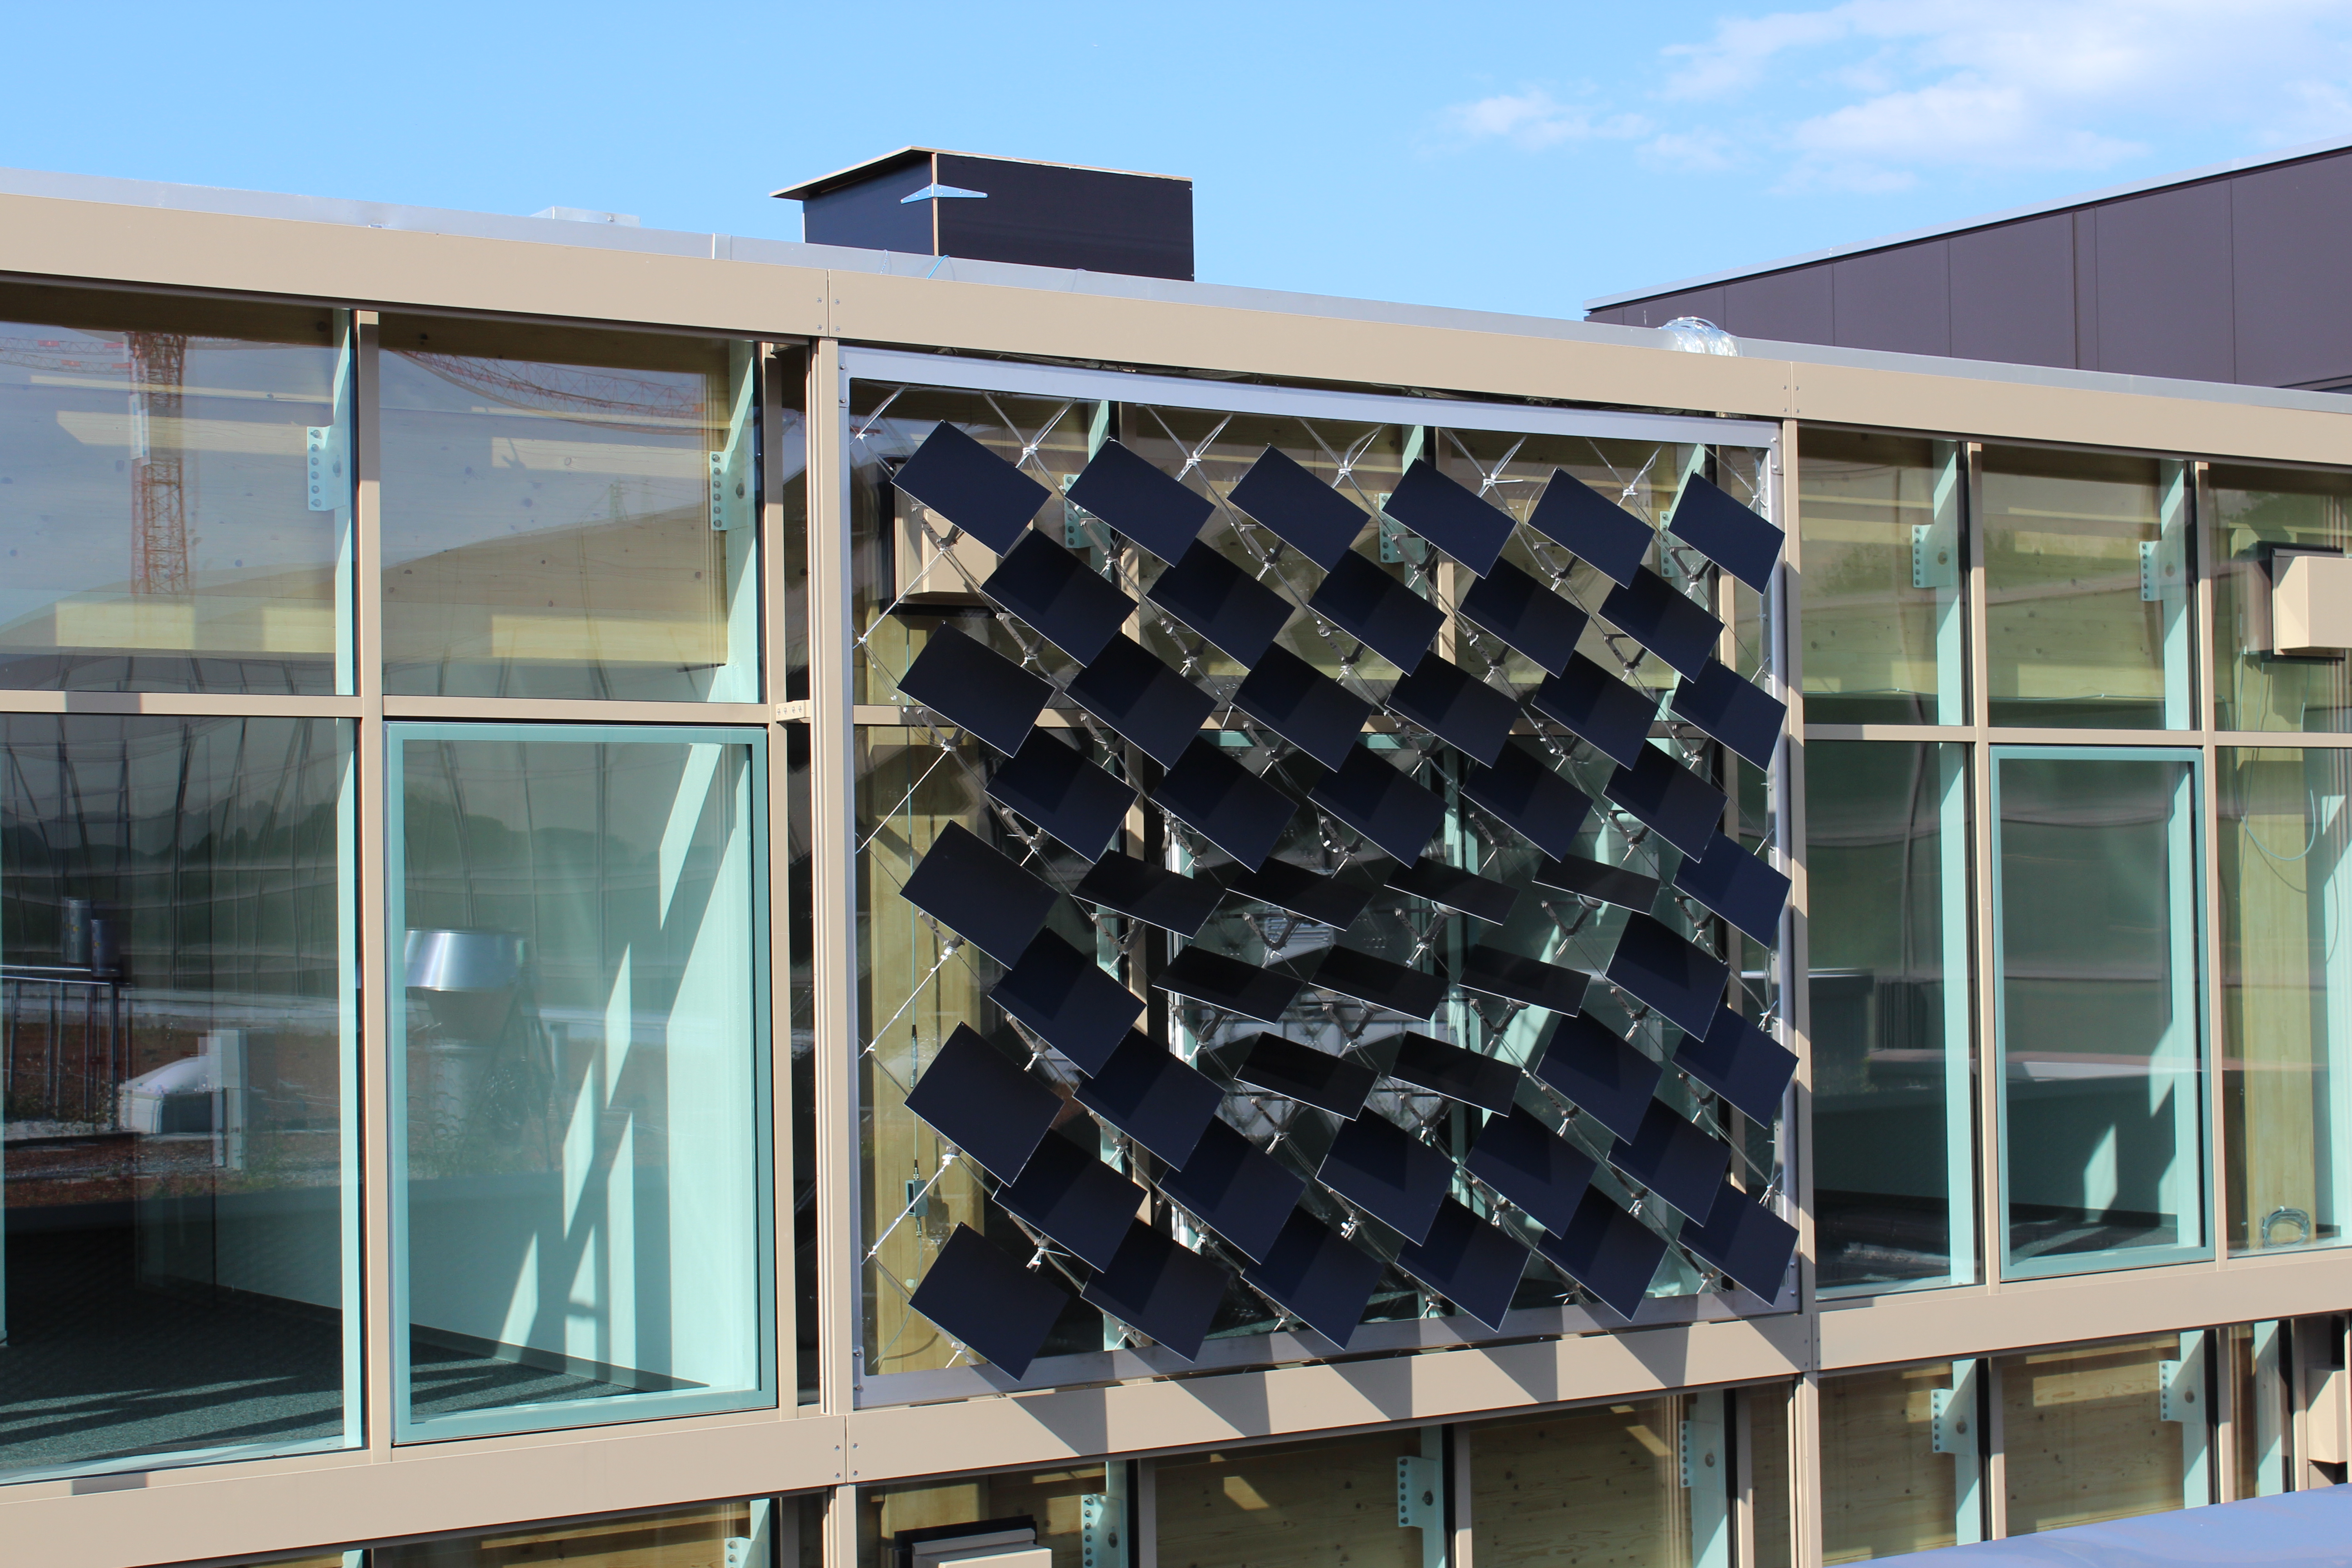
\includegraphics[width=8cm, trim= 0cm 0cm 0cm 0cm,clip]{honr.jpg}
\caption{An example of an ASF constructed at the House of Natural Resources \cite{nagy2015frontiers}}
\label{fig:HoNR}
\end{center}
\end{figure}

The design of an ASF comes at an added cost. The additional electronics, actuators, and supporting structure adds further embodied CO$_2$ to the product. It is therefore important to conduct a life cycle impact assessment (LCA) to analyse whether the carbon savings during operation offsets the increased embodied carbon emissions in manufacture. It is also important to see how variations in design can alter the GHG reduction potential of the technology. Aspects such as the chosen actuator, control system, and location of operation can have a significant impact on its environmental performance. There has already been work conducted on static photovoltaic systems \cite{raugei2007life}, however this has not yet been expanded to dynamic BIPV systems. \\

In this paper, we investigate the environmental performance of an ASF and compare it to existing static photovoltaic systems based off previous research \cite{raugei2007life}. We also investigate 1) Design variations of the ASF, 2) the operational emissions of a building, with and without an ASF, 3) its global and local environmental impact, and 4) the sensitivity of the LCA to its location and design


%In this paper we investigate the trade-off between added material and on-site energy production, along with other benefits such as adaptive shading. We assess 1) the ASF system with possible design variations, 2) the operation of a building with an ASF, 3) its global and local environmental impact, 4) the sensitivity of the LCA to the design and location, and 5) provide a comparison with existing static PV technologies. \\

The remainder of the paper is organized as follows. The next section introduces the ASF and the used LCA methodology. In Section \ref{ch:results}, we present the results of the LCA analysis. Section \ref{ch:discussion} discusses the results and provides design guidelines. Section \ref{ch:conclusion} concludes the paper.

\textcolor{cyan}{\textit{@Arno, Is the introduction too long?}}

% - In the last decades, building integrated photovoltaics (BIPV) have been adopted as part of the energy strategy towards 2050... \

% (advantages of BIPV, potential of BIPV)\\


% - The current developments of light-weight efficient thin film technologies have brought new design possibilities for architects in BIPV design... \

% (Adaptive Building Envelopes, examples, Envelope is the barrier between the internal and external environment, Advantages, seamless coupling with solar tracking mechanics) \\

% - One example of a multi functional facade that was recently released is the Adaptive Solar Facade.\\

% - The aim of this paper is to analyse the life cycle emissions of an adaptive solar facade and provide comparisons with standard shading systems and static BIPV solutions.\\


\section{Life cycle analysis methodology}
\label{ch:method}
% !TEX root = main.tex

In this section we detail the inventory, energy plus simulation methodology, important assumptions, and the LCA evaluation method. The assessment considers the environmental impacts of the production, operation, and disposal of an ASF. We assume a life time of 15 years \textcolor{cyan}{based on...}.
\\

\subsection{Life Cycle Inventory and Assumptions}

The mechanical components of the ASF can be broken into four parts: a PV panel, actuator, cantilever, and a cable net supporting structure. The PV panel, actuator and cantilever combine to form a dynamic PV module, which is then mounted on a cable net supporting structure. An exploded view of these components can be seen in Figure \ref{fig:explodedView}. There are also additional electronics which exists off the facade in a separate control box. Theses five components along with the assembly, are the main product systems in the manufacture of the ASF as seen in Figure \ref{fig:BOS}. 


% \begin{figure}[H]
% \begin{center}
% \includegraphics[width=8cm, trim= 0cm 0cm 0cm 0cm,clip]{ASFSubsystems.pdf}
% \caption{Breakdown of the ASF into six sub-product systems (Note change Steel frame to Suporting Structure, and Assembling ASF to Assembly. Also redraw this chart so it matches the subsubsections below)}
% \label{fig:subsystem}
% \end{center}
% \end{figure}

\begin{figure}[H]
\begin{center}
\includegraphics[width=8cm, trim= 0cm 0cm 0cm 0cm,clip]{explodedASFV2.png}
\caption{Exploded view of an ASF module mounted on a cable net supporting structure}
\label{fig:explodedView}
\end{center}
\end{figure}

\begin{figure}[ht]
\begin{center}
\includegraphics[width=14cm, trim= 0cm 0cm 0cm 0cm,clip]{BOS.pdf}
\caption{Breakdown of the ASF into five embodied product components and installation costs, operational costs, and disposal}
\label{fig:BOS}
\end{center}
\end{figure}
\textcolor{magenta}{\textit{(May Move the text to an Appendix and just keep the inventories)}}
\begin{description}

\item[PV Panel] \hfill\\
Weight is the primary restriction when selecting a PV panel. Any technology that requires glass encapsulation or a heavy substructure can therefore not be used. This limits us to CIGS and amorphous silicon panels.\\

CIGS PV panels was selected as the thin film panel of choice due to its high efficiency, low cost, and ability to be deposited on a polymer or aluminium substrate \cite{chirilua2011highly}. 

%A less efficient thin film amorphous silicon panel could also be used and will also be discussed in this analysis.\\

\textcolor{magenta}{\textit{(Not sure if it makes sense to provide the entire inventory here. If so, we would probably also need to give expected lifetimes, etc.)}}

% \begin{table}[H]
% \centering
% \begin{tabular}{lll}
% Panel Type  & SMQ    & ${\mathrm{\eta}}$  \\
% \hline
% CIGS 				& 0.7036 ${\mathrm{m^2_{panel}/m^2}}$ & 15\% \\
% a-Si				 	& 0.7036 ${\mathrm{m^2_{panel}/m^2}}$ & YY\%    \\
% Aluminum sheet 		& x ${\mathrm{kg/m^2}}$
% \end{tabular}
% \caption{Possible PV technologies for an ASF [Ref required]}
% \label{tab:PV}
% \end{table}

\begin{table}[H]
\centering
\begin{tabular}{ll}
\hline
Material description & SMQ \\ \hline
CIGS PV film       	 & 0.569 ${\mathrm{m^2_{PV}/m^2_{facade}}}$\\
Aluminum sheet 	 & 1.593 ${\mathrm{kg/m^2_{facade}}}$\\
Chromium steel panel adapter  & 1.422 ${\mathrm{kg/m^2_{facade}}}$\\
Polyethylene for junction box & 0.036 ${\mathrm{kg/m^2_{facade}}}$\\
Diode, glass for junction box & 0.011 ${\mathrm{kg/m^2_{facade}}}$\\
\hline
\end{tabular}
\caption{Inventory of a selection of top five input flows to the PV manufacturing process [ref required]}
\label{tab:PVinv}
\end{table}

\item[Actuator] \hfill \\
Traditionally photovoltaic actuation is done through the use of servo motors. Servo motors however become a limiting factor for adaptive facades due to their high upfront costs, and instability in heavy winds. Soft robotic actuators on the other hand are cheaper and more resilient to harsh environmental conditions\cite{Svetozarevic2014a}. The soft robotic actuators however are still in development and have a life time of five years. They will therefore require two rounds of maintenance during the lifetime of the ASF.
For the purpose of this analysis we will analyse both servo motors and soft robotic actuators. 

\begin{table}[H]
\centering
\begin{tabular}{ll}
\hline
Material description & SMQ \\ \hline
Chromium steel rings	 & 1.0665 ${\mathrm{kg/m^2_{facade}}}$ \\
Electronics, for control, 2-2way valves  & 0.0130  ${\mathrm{kg/m^2_{facade}}}$\\
Silicone chambers & 0.8887 ${\mathrm{kg/m^2_{facade}}}$\\
Polyurethane tubes &0.0933 ${\mathrm{kg/m^2_{facade}}}$\\
Air compressor, screw type, 0.75kW & NA ${\mathrm{kg/m^2_{facade}}}$\\
\hline
\end{tabular}
\caption{Inventory of four main input flows to the Actuator manufacturing process [ref required]}
\label{tab:ActuatorInv}
\end{table}

\item[Cantilever] \hfill \\
The cantilever is a steel connection point between the PV panel and the supporting structure.\\

\begin{table}[H]
\centering
\begin{tabular}{ll}
\hline
Material description & SMQ \\ \hline
Chromium steel bracket	 & 1.4220 ${\mathrm{kg/m^2_{facade}}}$ \\
Chromium steel fixing clamp  & 0.0284 ${\mathrm{kg/m^2_{facade}}}$\\
\hline
\end{tabular}
\caption{Inventory of main input flows to the Cantilever manufacturing process [ref required]}
\label{tab:CantileverInv}
\end{table}

\item[Supporting Structure] \hfill \\
The supporting structure is the connection point between the array of photovoltaic modules and the building itself. Many different designs are possible, however we will base our analysis of an adaptive solar facade that has already been constructed \cite{nagy2015frontiers}. This design consists of a steel cable-net that spans a steel supporting frame. The steel frame is then attached to the building itself.\\

\begin{table}[H]
\centering
\begin{tabular}{ll}
\hline
Material description & SMQ \\ \hline
Chromium steel L bar	 & 4.2581 ${\mathrm{kg/m^2_{facade}}}$ \\
Chromium steel U bar  & 2.7347 ${\mathrm{kg/m^2_{facade}}}$\\
Chromium steel swaged external thread  &0.2897 ${\mathrm{kg/m^2_{facade}}}$\\
Chromium steel wire rope WC  & 0.1593 ${\mathrm{kg/m^2_{facade}}}$\\
\hline
\end{tabular}
\caption{Inventory of the four main input flows to the manufacturing process of the Supporting Structure[ref required] \textcolor{cyan}{Could we change the L bar and U bar to Chromium Steel Frame? It is easier to understand}}
\label{tab:StructureInv}
\end{table}

\item[Control System and Electronics] \hfill \\
The control system is required for the actuation of panels and the regulation of photovoltaic electricity production.\\

\begin{table}[H]
\centering
\begin{tabular}{ll}
\hline
Material description & SMQ \\ \hline
Inverter 1.25kW	 & NA ${\mathrm{kg/m^2_{facade}}}$ \\
PV cable  & 3.1995 ${\mathrm{kg/m^2_{facade}}}$\\
Electronics control\footnote{c-Rio,8-slot, integrated 667Mhz}& 0.0419 ${\mathrm{kg/m^2_{facade}}}$\\
Electronics control\footnote{NI9476 32ch DO with cables and connectors}& 0.0097${\mathrm{kg/m^2_{facade}}}$\\
\hline
\end{tabular}
\caption{Inventory of the four main input flows to the manufacturing process of the Control System[ref required]}
\label{tab:ControlInv}
\end{table}

\item[Assembly] \hfill \\
There are many assembly options available. From past experience, an installation of an equivalent ASF required a hydraulic hoist which was in operation for eight hours \cite{jayathissa2015abs}. \\

\begin{table}[H]
\centering
\begin{tabular}{ll}
\hline
Material description & SMQ \\ \hline
Hoist, diesel  ${<}$18.64kW idling 8 hours & \textcolor{red}{NA} ${\mathrm{kg/m^2_{facade}}}$ \\
\hline
\end{tabular}
\caption{Inventory of main input flows to the Assembly Process[ref required] \textcolor{cyan}{Note that the 8 hours was for the HoNR ASF. We can scale this to get a value per sqm}}
\label{tab:AssemblyInv}
\end{table}

\end{description}

\subsection{Operational Emissions and Assumptions}
\label{ch:Meth:Opp}

The potential savings are based off previously completed numerical simulations \cite{jayathissa2015abs}. The simulation was conducted on a south facing office room. The room 7m meters in length, 4.9 meters wide and 3.1 meters high was modeled using Rhinoceros 3D CAD Package \cite{Rhino}. Grasshopper \cite{grasshopper} was used to model the dynamic aspects of the ASF which consists of an array of 400mm CIGS solar panels. The geometrical input is imported to Energy Plus \cite{energyplus} though the DIVA \cite{DIVA} interface. A single zone thermal analysis was conducted for each possible geometrical configuration of the ASF for each hour of the year. The results were then post processed in Python \cite{python} with the NumPy \cite{numpy}, and pandas \cite{pandas} plug-ins.\\

We conducted the simulation for three scenarios: 1) facade with no shading, 2) a facade with a static shading system angled at 45$^{\circ}$ to the horizontal axis, and 3) an adaptive solar facade. This analysis purely looks at the building energy performance through adaptive shading and doesn't include PV generation. \\

The building energy savings (kWh) are then converted to a GWP value based on the emission factor of the European Network of Transmission System Operators for Electricity (ENTSO-E) electricity mix (gCO2/kWh) \textcolor{blue}{[Add value and reference]}. \\

The energy required for actuation is also taken into account. It takes \textcolor{red}{0.15Wh} to fully open a single actuator. Based on the assumption of four full openings and closings per day, we approximate the energy requirement to be 174kWh in its lifetime. However as seen in Section \ref{ch:results}, this has a very small impact.\\

\begin{table}[H]
\centering
\begin{tabular}{ll}
\hline
\textbf{Building Settings}    &                                                \\
Office Envelope               & Roof: Adiabatic                                \\
                              & Floor: Adiabatic                               \\
                              & Walls: Adiabatic                               \\
                              & Window: Double Glazed LoE (e=0.2) 3mm/13mm air \\
                              & Floor Area: 21.7m2                             \\
Thermal Set Points            & Heating: 22$^{\circ}$ degrees Celcius                    \\
                              & Cooling: 26$^{\circ}$ degrees Celcius                    \\
Building System               & Hydronic Heating: COP=4                        \\
                              & Hydronic Cooling: COP=3                         \\
Lighting Control              & Lighting set point: 11.8W/m2                   \\
                              & Lighting Control: 300lx Threshhold           \\
                              & LED Lighting                                   \\
Occupancy                     & Office: Weekdays from 8:00-18:00               \\
                              & People set point: 0.1 persons/m2               \\
                              & Infiltration: 0.5 per hour                     \\
                              &                                                \\
\textbf{Location Assumptions} &                                                \\
Weather File                  & Geneva, Switzerland (067000IWEC)              \\
Electricity Mix               & ENTSO-E\cite{itten2012life}                                           \\
                              &                                                \\
\textbf{Maintenance}          &                                                \\
Actuator Replacements         & Every 5 years                                  \\
                              &                                                \\
\textbf{ASF Settings}         &                                                \\
Full open and closes per day  & 4 per day                                      \\
\hline
\end{tabular}
\caption{Summary of main assumptions for the calculation of operational emissions}
\label{tab:AssumptionsOpp}
\end{table}


% Maybe have a reference case here, see previous commits 

\subsection{Evaluation Method}
The life cycle analysis is performed according to the ISO 14040 and ISO 14044 and is performed in five stages 1) goal, 2) scope definition, 3) inventory analysis, 4) impact assessment and 5) interpretation.\\ % 15804 to be discussed

\begin{description}
\item[Goal:] This paper assesses carbon emission reductions, therefore the impact category used is the global warming potential (GWP\textcolor{magenta}{\textit{[IPCC 2013 reference - let me know if you need it]}}). This is described as the emissions of ${\mathrm{gCO_2-eq}}$ divided by the electricity produced in kWh. This is also known as the emission factor (gCO$_2$/kWh) which is expressed in Equation \ref{eq:EF} where ($G$) is the electricity production in (kWh). This analysis will also touch on the regional distributions of GWP and terrestrial acidification to give a complete picture.

\begin{equation}
EF=\frac{{\sum GWP}}{\mathrm{G}}
\label{eq:EF}
\end{equation}

\item[Scope:] The GWP scope consist of Embodied Energy ($GWP_{Em}$), Dynamic Actuation ($GWP_{Act}$), Maintenance ($GWP_{M}$), and Disposal ($GWP_{Disp}$). The GWP savings through adaptive shading ($GWP_{Opp}$) are subtracted to produce our final GWP. This scope is summarised in Figure \ref{fig:BOS}.

\begin{equation}
\sum GWP={\mathrm{GWP_{Em}  + GWP_{Act} + GWP_{M} + GWP_{Disp} - GWP_{Opp} }}
\label{eq:GWP}
\end{equation}

% The functional unit needs to be based on the primary function of the technology. For adaptive building integrated photovoltaics this function can be twofold. When the adaptive BIPV acts as a shading system in front of a glass facade area the functional unit of ${\mathrm{m^2}}$ is used, while a comparison with static facade mounted photovoltaic systems requires the functional unit of electricity produced in ${\mathrm{kWh}}$. \textcolor{magenta}{\textit{(We should discuss the functional unit again. It should be defined more precisely / comprehensively.)}}



% In our assessment, we want to obtain the emission factor (gCO$_2$/kWh) of an ASF as expressed in Equation \ref{eq:EF}. 




The electricity produced, G, in kWh is expressed in Equation \ref{eq:solar} based off International Energy Agency standards [REF REQUIRED]. \textit{I} is the Irradiation \textcolor{red}{(unit)}, ${\eta}$ is the conversion efficiency, \textit{PR} is the performance ratio, \textit{LT} is the service life \textcolor{red}{(unit)}, and \textit{A} is the module area \textcolor{red}{(unit)}.

\begin{equation}
G=\frac{{\mathrm{GWP}}}{{\mathrm{I \cdot \eta  \cdot PR \cdot LT \cdot A}}}
% what is G
\label{eq:solar}
\end{equation}


% The scope of the LCA comprises of the embodied, operational, and disposal global warming impact of the respective system. Figure \ref{fig:BOS} illustrates the system boundaries of the process flows. The supporting structures are also included in the system boundaries. The reason for this is that technologies within the building envelope also change the design of the supporting structures. The supporting structure of solar panels is referred to as balance of systems (BOS).\\

\item[Inventory:] The inventory data was obtained through technical drawings, research papers describing the technology and expert judgement. The Ecoinvent v3.1 database is used as the main LCI database \cite{frischknecht2005ecoinvent}. To keep assumptions consistent, only data from this database is used. \textcolor{magenta}{\textit{(Is that so? Didn't we add a CIGS dataset?)}} Furthermore, the cut-off approach is used for the allocation of recycling and landfill disposal. This means that recycling does not generate any credit for the product and resulting benefits are not taken into account. Furthermore the use of recycled products do not bear the burden of processes higher up the chain.\textcolor{magenta}{\textit{(We don't do any system expansion?)}}\\



\item[Assessment:] For the impact assessment the ReciPe midpoint (H) indicator is used \cite{zelm2009recipe}. \textcolor{magenta}{\textit{(This is a little inconsistent. We should consistently use the term environmental impact as opposed to carbon content, etc.)}} \textcolor{blue}{@Niko, I don't understand what is inconsistent here? Could you suggest some text for this paragraphs?}The impact assessment is performed using the OpenLCA impact assessment tool \cite{ciroth2007ict}. The results of the assessment will be compared with the emission factor of other PV systems \cite{raugei2007life}\\
	% we may need to discuss system expansion
	% PV electricity production not included?

% what LCI DB (ecoinvent) is used? refer to Annex?
% see above. Explain what is included and excluded

\end{description}

\subsection{Sensitivity Analysis}

In order to evaluate the impact of varying parameters on the LCA, we performed a sensitivity analysis on the following assumptions
\begin{itemize}
\item The GWP of the electricity mix
\item The type of actuation system (servo motors compared to soft robotic actuators)
\item The complexity of the control system
\item The uncertainty in the eco-invent background system (Monte Carlo Analysis)
\end{itemize}

% The inputs are summarised in Table \ref{tab:sens}

% \begin{table}
% \centering
% \begin{tabular}{lll}
% Assumption & Case A & Case B \\
% \hline
% Electricity Mix  & Switzerland & Germany \\
% Control System  & Controlling rows of panels        & Controlling individual panels    \\
% Actuator Type           & Servo Motor       & Soft Robotic Actuator   \\
% \end{tabular}
% \caption{Inputs to the Sensitivity Analysis Conducted}
% \label{tab:sens}
% \end{table}

\section{Environmental Performance of the Adaptive Solar Facade}
\label{ch:profile}
\input{3_profile}

\section{Comparison to other technologies}
\label{ch:comparison}
% !TEX root = main.tex




\subsection{Comparison to existing PV technologies}

Comparison of the ASF to other PV technologies and the UCTE electricity mix is highlighted in Figure \ref{fig:compPV}. We can see in this figure that the ASF without shading benefits is inferior to all other technologies. It is only with the added shading benefits that we really see the advantages of the adaptive system. \textcolor{magenta}{\textit{(I think we need to provide and explain the e+ simulation results somehwere.)}}
We can also see that the utilisation of the ASF in an area where the electricity mix has low GWP intensity such as Switzerland also has disadvantages. It is capable of out performing Silicone based technologies but is still inferior to simply mounted CIGS panels. Note that even the panels themselves of the ASF, without the BOS, is still lower that the CIGS installation. This is due to the added inefficiencies as the panels are not always at the optimum position to the sun.


\begin{figure}[H]
\begin{center}
\includegraphics[width=10cm, trim= 0cm 0cm 0cm 0cm,clip]{compPV.pdf}
\caption{Comparison of thin-film and BOS to other PV technologies. I would add some extra columns, one without shading, one with the ASF in Switzerland, one with the ASF in Europe}
\label{fig:compPV}
\end{center}
\end{figure}






\section{Discussion}
\label{ch:discussion}
\input{5_discussion}

\section{Conclusion}
\label{ch:conclusion}
% !TEX root = main.tex

The environmental performance of the ASF has been shown to be favorably competitive with a classic BIPV installation. Even though the embodied environmental performance is \textcolor{red}{six times} worse than a static CIGS installation, it is offset three fold through adaptive shading. This combination of adaptive shading with photovoltaic generation brings new advantages to solar as it effectively has a negative emission factor of \textcolor{red}{-470.1 g CO2/kWh}. These advantages however, will not be present if the ASF is installed over an opaque building surface. It is therefore better to install static systems over opaque facades, and keep the adaptive system for glazed facades only. \\
The design of an ASF naturally can greatly influence the results. The use of soft robotic actuators over servo motors increases the environnmental performance by \textcolor{red}{60 kgCO2} per square meter. The control electronics, which represents 11\% of the total embodied emissions, can increase by \textcolor{red}{35\%} if we increase the resolution of the facade so each panel can move independently. Also the supporting structure, representing \textcolor{red}{20\%} of total emissions can be better optimised to use less steel, or an alternative material. \\
The emission factor of the grid electricity mix also varies greatly between countries and has a large influence on the savings through adaptive shading. The reductions in heating, cooling and lighting of an office room will have CO2 savings based on the electricity mix. In a country with low CO2 grid mix, such as Switzerland, will only see \textcolor{red}{140kgCO2/sqm$_{facade}$} reductions. In Germany on the other hand, there will be operational savings of \textcolor{red}{700kgCO2/sqm$_{facade}$}.\\
Ultimately we see that the combination of BIPV systems and adaptive shading, compliment each other nicely. We see an improvement in environmental performance of the PV technology, and open up new architectural possibilities for the aesthetic integration of PV panels over glazed building surfaces.




\section{Acknowledgments}
\label{ch:acknowledgments}
% !TEX root = main.tex

The authors would like to acknowledge the HiLo and HoNR project members for the design and construction of the ASF: Supermanoeuvre (Sydney Australia) and the Professorship of Architecture and Structures (BRG, ETH Zürich) for their work in designing the HiLo building; and the Institute of Structural Engineering (IBK, ETH Zürich) for their work in designing the HoNR building. The authors would also like to thank other key contributors to the ASF Project: Bratislav Svetozarevic, Moritz Begle, Johannes Hofer, Nicola Offeddu, and Giovanni Bianchi. \\

Funding for the conduction of the research came from the Building Technologies Accelerator program of Climate-KIC.

%% appendix sections are then done as normal sections
%% \appendix
%% \section{}
%% \label{}

%% bibitems, please use
  \bibliographystyle{elsarticle-num} 
  \bibliography{references}

\end{document}
\endinput